\documentclass[a4paper]{article}

\usepackage[utf8]{inputenc}
\usepackage[portuges]{babel}
\usepackage{graphicx}
\usepackage{a4wide}
\usepackage[pdftex]{hyperref}
\usepackage{float}
\usepackage{indentfirst}
%\usepackage{subcaption}
\usepackage{subfig}
\usepackage{fancyhdr}

\pagestyle{fancy}
\fancyhf{}
\rhead{TP3 - Grupo 56}
\lhead{Questões e Respostas}
\rfoot{Page \thepage}

\begin{document}

\title{TP3 - Camada de ligação lógica: Ethernet e Protocolo ARP\\ Redes e Computadores\\Grupo 56}
\author{Bruno Martins (a80410) \and Filipe Monteiro (a80229) \and Márcio Sousa (a82400)}
\date{\today}

\begin{titlepage}

  %título
  \thispagestyle{empty}
  \begin{center}
  \begin{minipage}{0.75\linewidth}
      \centering
  %engenharia logo
     % 
\includegraphics[width=0.4\textwidth]{imgs/eng.jpeg}\par\vspace{1cm}
      \vspace{1.5cm}
  %titulos
      \href{https://www.uminho.pt/PT}{\scshape\LARGE Universidade do Minho} \par
      \vspace{1cm}
      \href{https://www.di.uminho.pt/}{\scshape\Large Departamento de Informática} \par
      \vspace{1.5cm}

  \maketitle
  \end{minipage}
  \end{center}

  \vspace{2cm}

  


  \clearpage

 \end{titlepage}
 \tableofcontents
 
 \section{Captura e Análise de Tramas Ethernet}
 \subsection{Anote os endereços MAC de	origem e de	destino	da trama capturada.}
\begin{figure}[H]
\centering
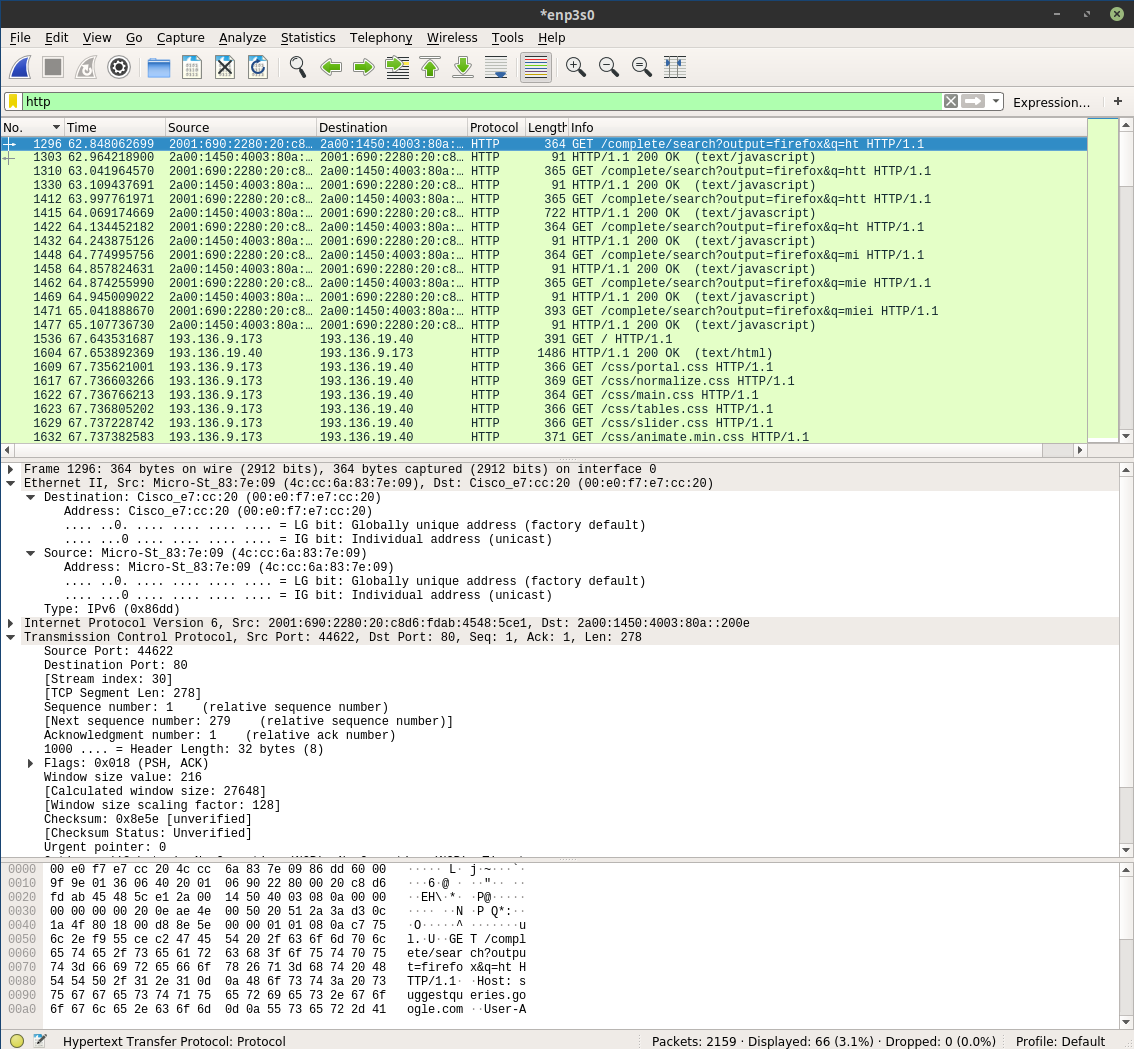
\includegraphics[scale=0.30]{pics/wireshark-p1.png}
\caption{Primeiro trama capturada ao aceder à página miei.di.uminho.pt}
\end{figure}
 O endereço MAC de origem é \underline{4c:cc:6a:83:7e:09}.\newline
 O endereço MAC do destino é \underline{00:0a:8a:97:74:80}.


 \subsection{Identifique	a	que	sistemas	se	referem. Justifique.}
\begin{figure}[H]%
    \centering
    \subfloat[Em cima, o IP da nossa máquina (inet) assim como o endereço MAC (ether). Em baixo apresenta o IP correspondente à página da \textit{web} em questão.]{{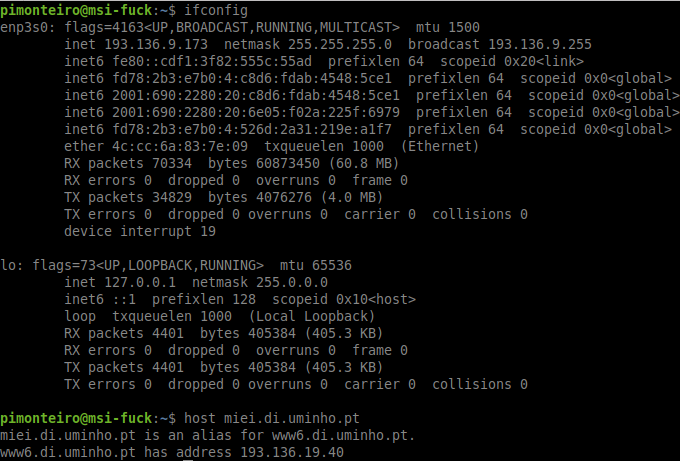
\includegraphics[scale=0.5]{pics/p2.png}}}%
    \qquad
    \subfloat[Endereços MAC do \textit{host} (nossa máquina) e do servidor.]{{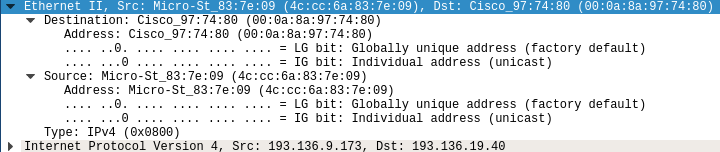
\includegraphics[scale=0.5]{pics/p2-1.png}}}%
    \caption{Validação dos endereços de cada máquina.}%
    \label{fig:example}%
\end{figure}
 
 O endereço MAC de origem corresponde à nossa máquina. 
 O endereço MAC de destino refere-se ao servidor destino (\textit{website}).
 
 \subsection{Qual o	valor hexadecimal do campo Type da trama Ethernet? O que significa?}
 \begin{figure}[H]
\centering
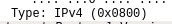
\includegraphics[scale=0.60]{pics/p3.png}
\caption{Detalhes do campo \textit{Type} do trama \textit{Ethernet}.}
\end{figure}
 O valor hexadecimal é  0x0800 e significa que o tipo é IPv4.
 
 \subsection{Quantos bytes são	usados desde	o	início	da	trama até	ao	caractere	ASCII	“G”	do	
método HTTP	GET? Calcule	e	indique,	em	percentagem,	a	sobrecarga (overhead)	
introduzida pela	pilha	protocolar no	envio	do	HTTP	GET.}
\begin{figure}[H]
\centering
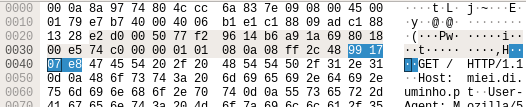
\includegraphics[scale=0.60]{pics/p4.png}
\caption{Frame da trama. A seguir ao selecionado começam os dados.}
\end{figure}
Existem 66 bytes de \textit{overhead}. No total do pacote existem 391 bytes. A percentagem de overhead é aproximadamente 16,8\%.
 
 \subsection{Através	 de	 visualização	 direta	 de	 uma	 trama	 capturada,	 verifique	 que,	
possivelmente, o	 campo	 FCS	 (Frame	 Check	 Sequence) usado	 para	 deteção	 de	
erros	não	está	a	ser	usado.	Em	sua	opinião, porque	será?}
O campo FCS não está a ser usado porque como o campo FCS ocupa bastante espaço no datagrama e o protocolo Ethernet já é atualmente mais fiável que no passado, não se envia este, sendo que se for preciso reenvia-se um novo pacote. 

\subsection{Qual	 é	 o	 endereço	 Ethernet da	 fonte?	 A	 que	 sistema	 de	 rede	 corresponde?	
Justifique}
\begin{figure}[H]
\centering
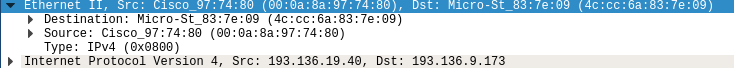
\includegraphics[scale=0.50]{pics/p6.png}
\caption{Trama \textit{Ethernet} com os endereços MAC da fonte e do destino, assim como os IP's respetivos.}
\end{figure}
O endereço Ethernet da fonte é 00:0a:8a:97:74:80 e corresponde ao router que faz a ligação a uma rede exterior, pois o servidor não se encontra na nossa sub-rede, logo o MAC Address não pode pertencer ao servidor, mas sim ao aparelho de conexão à rede onde se contra o servidor.

\subsection{Qual	é	o	endereço	MAC	do	destino?	A	que	sistema	corresponde?}
\begin{figure}[H]
\centering
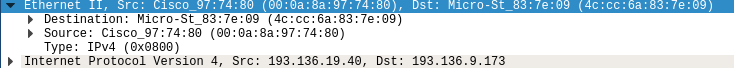
\includegraphics[scale=0.50]{pics/p6.png}
\caption{Trama \textit{Ethernet} com os endereços MAC da fonte e do destino, assim como os IP's respetivos.}
\end{figure}
O enderço MAC destino é 4c:cc:6a:83:7e:09 e corresponde à nossa máquina.


\subsection{Atendendo	ao	conceito	de	desencapsulamento	protocolar,	identifique	 os	 vários	
protocolos	contidos	na	trama	recebida.}
\begin{figure}[H]
\centering
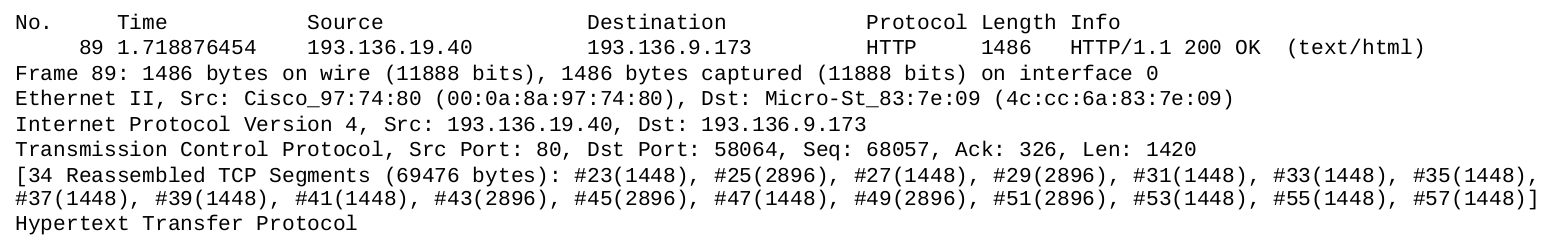
\includegraphics[scale=0.30]{pics/p8.png}
\caption{Diferentes encapsulamentos protocolares da trama recebida.}
\end{figure}
Temos TCP, IPv4, HTTP, Ethernet II.

\section{Protocolo Arp}
\setcounter{subsection}{8}

\subsection{Observe o conteúdo da tabela ARP. Diga o que significa cada uma das colunas}
\begin{figure}[H]
\centering
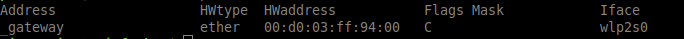
\includegraphics[scale=0.50]{pics/p9.png}
\caption{Tabela ARP da nossa máquina.}
\end{figure}

\begin{enumerate}
    \item \textit{Address} - IP/endereço de uma máquina;
    \item \textit{HWtype} - tipo de ligação com essa máquina;
    \item \textit{HWaddress} - endereço MAC correspondente;
    \item \textit{Flags} - indicam o estado da entrada, ou seja, se foi deduzido, inserido manualmente ou incompleto;
    \item \textit{Iface} - indica o nome da \textit{interface} a que o dispositivo está conectado.
\end{enumerate}



\subsection{Qual é o valor hexadecimal dos endereços origem e destino na trama Ethernet
que contém a mensagem com o pedido ARP (ARP Request)? Como interpreta e
justifica o endereço destino usado?}
\begin{figure}[H]
\centering
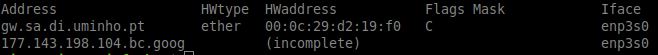
\includegraphics[scale=0.50]{pics/p10.png}
\caption{Tabela ARP da nossa máquina após conexão ao servidor.}
\end{figure}
Endereço origem: 4c:cc:6a:83:7e:09
Endereço destino: ff:ff:ff:ff:ff:ff 

O endereço destino é este pois o pedido \textit{ARP Request} usa um endereço MAC de broadcast para todas as máquinas receberem o pacote e eventualmente alguma aceitar, tratar e responder (por ser o IP destino do pacote).

Neste caso, fizemos um \textbf{ping 192.168.100.198}, não estando este guardado na tabela de ARP antes do ping.

\subsection{Qual o valor hexadecimal do campo tipo da trama Ethernet? O que indica?}
\begin{figure}[H]
\centering
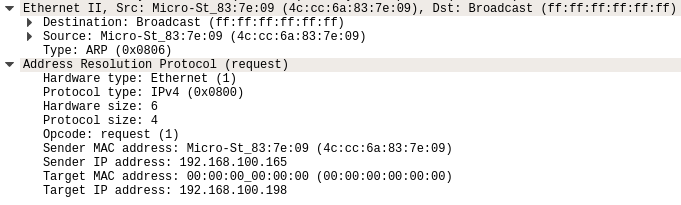
\includegraphics[scale=0.540]{pics/p10-1.png}
\caption{Trama c}
\end{figure}
O valor do campo tipo da trama é de 0x0806 que indica ser um ARP, sendo um ARP Request se analisarmos o \textit{opcode}.

\subsection{Qual o valor do campo ARP opcode? O que especifica? Se necessário, consulte a RFC do protocolo ARP \url{http://tools.ietf.org/html/rfc826.html}}
O valor do campo ARP \textit{opcode} é 1 e significa que se trata de um \textit{Arp Request}.

\subsection{Identifique  que  tipo  de  endereços  estão  contidos  na  mensagem  ARP? Que conclui?}
Na mensagem ARP estão contidos dois tipos de endereços: endereços MAC e endereços IP, que serão usados para encaminhar o pacote para o destino correto e para mais tarde serem adicionados à tabela ARP.


\subsection{Explicite que tipo de pedido ou pergunta é feita pelo host de origem?}
O \textit{host} de origem pede a quem tiver o IP XXX.XXX.XXX.XXX para lhe responder, ficando assim a saber o  endereço MAC da máquina destino.


\subsection{Localize a mensagem ARP que é a resposta ao pedido ARP efectuado.}

\begin{enumerate}
    \item \underline{Qual o valor do campo ARP opcode? O que especifica?}\newline\newline
    O valor do campo ARP \textit{opcode} é de 2 que significa ser uma resposta da máquina a um pedido ARP.\newline
    \item \underline{Em que posição da mensagem ARP está a resposta ao pedido ARP?}\newline\newline
    \begin{figure}[H]
    \centering
    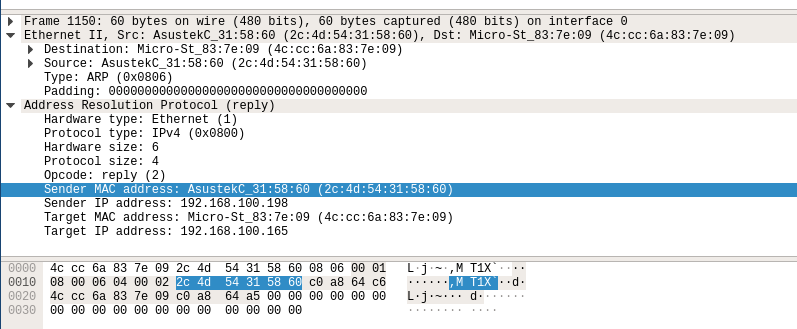
\includegraphics[scale=0.40]{pics/p15-1.png}
    \caption{Ping de n1 para n2 (canto superior esquerdo), \textit{tcpdump} de n2 (canto superior direito), \textit{tcpdump} de n3 (canto inferior esquerdo), \textit{tcpdump} de n4 (canto inferior direito}
    \end{figure}
    A resposta encontra-se não entre os \textit{bytes} 23 e 28 (campo \textit{MAC Address}).
\end{enumerate}


\section{ARP Gratuito}
\setcounter{subsection}{15}

\subsection{Identifique um pacote de pedido ARP gratuito originado pelo seu sistema. Analise o conteúdo de um pedido ARP gratuito e identifique em que se distingue dos  restantes  pedidos  ARP. Registe a trama Ethernet correspondente. Qual o resultado esperado face ao pedido ARP gratuito enviado?}
\begin{figure}[H]
\centering
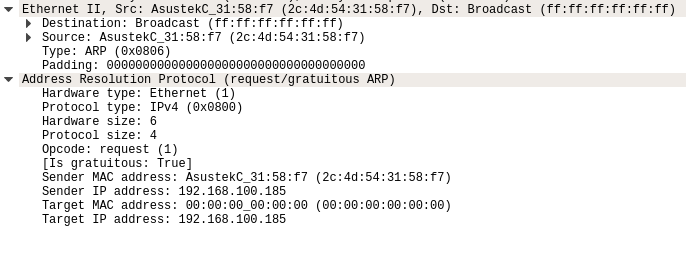
\includegraphics[scale=0.50]{pics/p162.png}
\caption{Pedido ARP gratuito} % ver legenda
\end{figure}
O pedido ARP gratuito distingue-se dos outros porque o Sender IP e o Target IP são o mesmo, o que não acontece normalmente.


\section{Domínio de Colisão}
\setcounter{subsection}{16}

\subsection{Faça ping de n1 para n2. Verifique com a opção tcpdump como flui o tráfego nas diversas interfaces dos vários dispositivos. Que conclui?}
\begin{figure}[H]
\centering
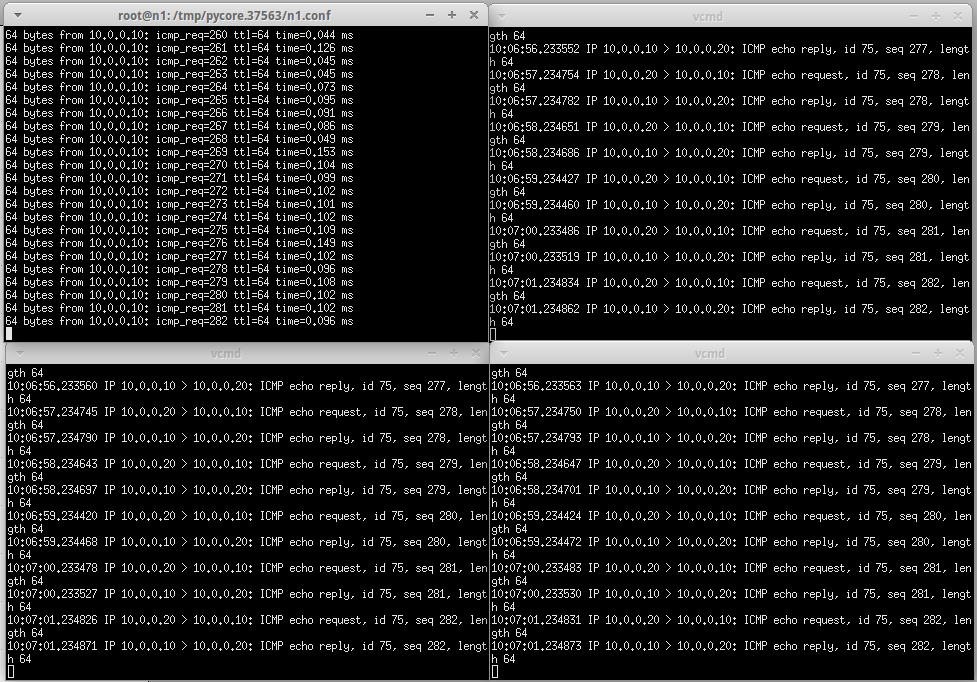
\includegraphics[scale=0.40]{pics/p17.png}
\caption{Ping de n1 para n2 (canto superior esquerdo), \textit{tcpdump} de n2 (canto superior direito), \textit{tcpdump} de n3 (canto inferior esquerdo), \textit{tcpdump} de n4 (canto inferior direito} % ver legenda
\end{figure}
Analisando o tráfego, concluimos que com \textit{hub}, apesar de estarmos a enviar tráfego de n1 para n2, os outros dispositivos conseguem ver este tráfego. Existe também a possibilidade de colisões, podendo haver a eliminação de pacotes, sendo depois necessário o seu reenvio. Para prevenir esta colisões existe o protocolo CSMA/CD que obriga dispositivos a esperar que outro acabe de comunicar antes de tentarem mandar tráfego.


\subsection{Na topologia de rede substitua o hub por um switch. Repita os procedimentos que realizou na pergunta anterior. Comente os resultados obtidos quanto à utilização de hubs e switches no contexto de controlar ou dividir domínios de colisão. Documente as suas observações e conclusões com base no tráfego observado/capturado.}
\begin{figure}[H]
\centering
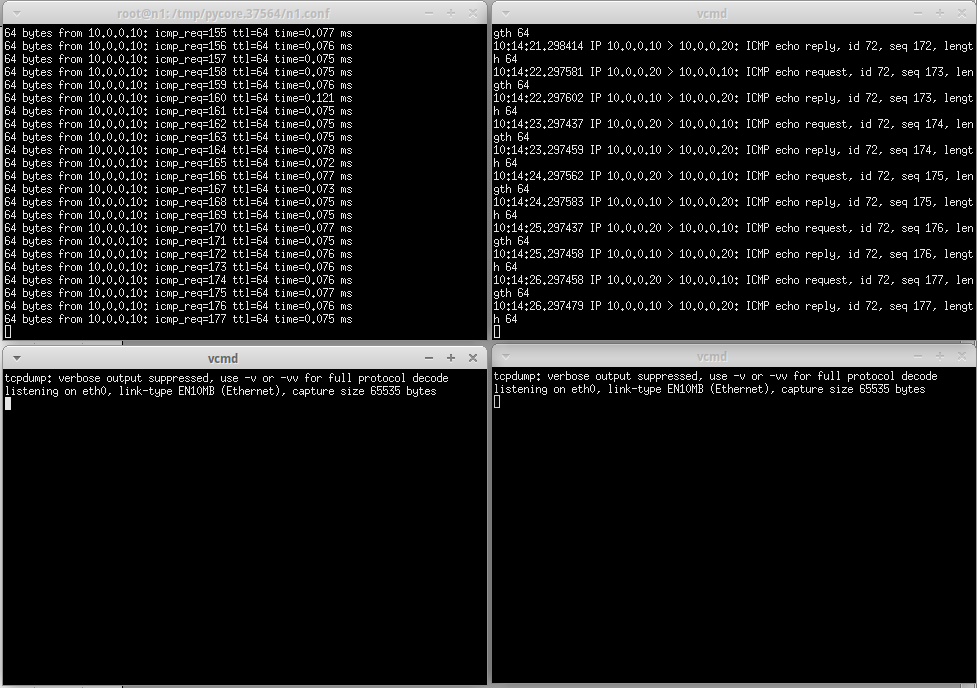
\includegraphics[scale=0.40]{pics/p18.png}
\caption{Ping de n1 para n2 (canto superior esquerdo), \textit{tcpdump} de n2 (canto superior direito), \textit{tcpdump} de n3 (canto inferior esquerdo), \textit{tcpdump} de n4 (canto inferior direito} % ver legenda
\end{figure}
Utilizando um \textit{switch} ao invés de \textit{hub}, a rede o tráfedo de um dispositivo para outro passa a ir diretamente da origem para o destino, sendo que os outros dispositivos na rede não conseguem ver tráfego entre estes dois (o \textit{switch} encaminha o pacote diretamente para a porta onde se encontra o destino).

\section{Conclusão}
Este relatório tem como objetivo appresentar as respostas à ficha apresentada nas aulas práticas. A resolução desta ficha permitiu-nos adquirir conhecimento acerca da arquitetura Ethernet fazendo com que, na prática, vissemos os endereços MAC de origem e destino das tramas que capturavamos utilizando o software \textit{Wireshark} que nos ofereceu uma visão mais realista. Um dos grandes focos desta ficha foi também o protocolo ARP encontrado ao nível da ligação de dados, em que numa primeira fase foi analizado o conteúdo da tabela ARP, bem como os edereços lá especificados e o seu processo de encaminhamento de tramas. Já numa fase mais avançada foi forçado um pedido ARP gratuito de forma a conseguir visualizar as diferenças entre ele e os restantes pedidos. No final, através de uma topologia modelada no \textit{CORE}, foi possível analisar as diferenças entre \textit{hubs} \textit{switches} dentro de uma rede, como funcionam e o porquê de os \textit{switches} serem uma melhor escolha para usar.

\end{document}
